\documentclass[11pt]{scrartcl}
\usepackage[utf8]{inputenc}
\usepackage{evank}


%% insert title here
\newcommand{\titlee}{Relativity II [Solutions]}
\parindent 0 pt

\title{\titlee}
\author{Cambridge Physics Academy}
\date{2023-2024}


\begin{document}

\thispagestyle{empty}
\begin{center}
    
    
    \Huge \textbf{\textsf{\titlee}}

    \large \theauthor
\end{center}

\setcounter{section}{-1}
\section{Readings}
\begin{itemize}
    \item Chapter 12 of Morin
\end{itemize}
Feel free to do problems from the readings as extra practice.


\section{Lecture review}
\begin{defn}[Energy and Momentum]
The energy $E$ and momentum $\mathbf p$ respectively of a particle moving at speed $v$ with $\gamma=\sqrt{1-v^2}$ are $$E=\gamma m\qquad \mathbf p=\gamma m\mathbf v$$It can be seen that energy and momentum follow two important relations: $$E^2-p^2=m^2\qquad v=\frac{p}{E}$$If the primed frame moves at a speed $+v$ in the lab frame, the Lorentz transformations of $E$ and $p$ are \begin{gather*}
    E=\gamma (E'+vp')\\
    p=\gamma(p'+vE')
\end{gather*}
\end{defn}
\begin{defn}[4-momentum]
The energy-momentum 4-vector (or 4-momentum) is defined as $$P=(E,\mathbf p)=(E,p_x,p_y,p_z)$$
The dot product of two 4-vectors $P_1=(a_1,\mathbf b_1)$ and $P_2=(a_2,\mathbf b_2)$ is defined as $$P_1P_2=a_1a_2-\mathbf b_1\cdot \mathbf b_2$$
\end{defn}
\begin{theorem}[Properties of 4-momentum]
Three key properties of 4-momentum you should remember: \begin{enumerate}
    \item $P^2=m^2$
    \item The inner product of two 4-momenta $P_1P_2$ in any given frame is invariant under the Lorentz transformations.
    \item During collisions and decays, the total 4-momentum is conserved.
\end{enumerate}
\end{theorem}
\begin{defn}[Photons]
Photons are massless light particles. In units of $c=1$, the energy and momentum of a photon are equal: $E=p$. The energy of a photon can be related to its frequency $f$ as $E=hf$, and its momentum can be related to its wavelength $\lambda$ as $p=h/\lambda$. It can be seen that the relation $f\lambda=c$ holds. 
\end{defn}
\begin{defn}[Force]
Force is defined as $$\mathbf F=\frac{d\mathbf p}{dt}$$It can be shown via taking the derivative that a force applied in the direction of motion is related to acceleration by $$F=\gamma^3 ma$$The transformations of $F$ are \begin{gather*}F_\parallel=F_\parallel'\\
F_\perp = \frac{F_\perp'}{\gamma}\end{gather*}
\end{defn}

\section{Problem Set}

\subsection{Exercises}

\begin{prob}
    During lecture, we found answers for problems with $c=1$. However, it's good practice on exams to put $c$ back in. Fix the units of the following answers derived in class: $$v=\frac{p_{total}}{E_{total}}\qquad \sigma=\frac 32 v^2\qquad \lambda'=\lambda+\frac hm(1-\cos\theta)\qquad t=\sqrt{x^2-\frac{m^2}{F^2}}$$ 
    For the rest of this homework, leave your answers with $c=1$. 
\end{prob}

\begin{sol}
    The modified answers are $$v=\frac{p_{total}c^2}{E_{total}}\qquad \sigma=\frac 32 \frac{v^2}{c^2}\qquad \lambda'=\lambda+\frac h{mc}(1-\cos\theta)\qquad t=\sqrt{\frac{x^2}{c^2}-\frac{m^2c}{F^2}}$$ 
\end{sol}

\begin{prob}
    Two masses $m$ move at opposite speeds $v$ in the lab frame. What is the energy of one mass in the rest frame of the other?
\end{prob}

\begin{sol}
    One way is to use velocity addition, but you can also use 4-momentum. In the lab frame, $P_1P_2=(\gamma m,\gamma mv)\cdot(\gamma m,-\gamma mv)=\gamma^2m^2(1+v^2)$. In the rest frame of one of the masses, if the energy of the other is $E$, then $P_1'P_2'=(m,0)\cdot (E,p)=Em$. The dot product is Lorentz invariant, so equating the two results we get $$E=\gamma^2m(1+v^2)=\boxed{\frac{1+v^2}{1-v^2}m}$$
\end{sol}

\begin{prob}
    A mass $m$ decays into four photons, three of which travel in directions orthogonal to one another. What is the momentum of the last photon?
\end{prob}

\begin{sol}
    If the energy of the three orthogonal photons are $E$, then the last photon must have energy $E\sqrt 3$ (remember that $E=p$). As a result, $E(3+\sqrt 3)=m$, so $$p=E\sqrt 3=\boxed{\frac{m}{\sqrt 3+1}}$$
\end{sol}

\begin{prob}
    A mass $m_A$ is traveling at speed $v$ in the positive $x$-direction when it collides with a mass $m_B$ initially at rest. Assume in this problem that after the collision, the masses of the two objects are still $m_A$ and $m_B$. If $m_B$ scatters in the positive $y$-direction with energy $E_B$, find the angle that $m_A$'s resulting path makes with the $x$-axis.
\end{prob}

\begin{sol}
    By conservation of energy, the energy of $m_A$ after the collision must be $E_A=\gamma m_A+m_B-E_B$. Its momentum in the vertical direction is equal to $p_{Ay}=-p_B=\sqrt{E_B^2-m_B^2}$. Its total momentum can be found via $p_A=\sqrt{E_A^2-m_A^2}.$ Thus the angle made to the $x$-axis is $$\theta=\sin^{-1}\left(-\frac{p_B}{p_A}\right)=\boxed{\sin^{-1}\left(-\frac{\sqrt{E_B^2-m_B^2}}{\sqrt{(\gamma m_A+m_B-E_B)^2-m_A^2}}\right)}$$
\end{sol}

\begin{prob}
    Mass $m_A$ starts at rest. Consider the following decay chain: $$m_A\rightarrow m_B+m_B\rightarrow \gamma+\gamma+m_B$$ What is the maximum possible energy of one of the photons?
\end{prob}



\begin{sol}
The two photons will carry the energy and momentum of one of the $m_B$'s after the decay. To maximize the energy of one of the photons, we minimize that of the other. Thus in the maximum case both photons will travel along the direction of motion of $m_B$. To be concrete, let the 4-momentum of $m_B$ be $P_B=(E_B,p_B,0,0)$, where we have set the $x$ axis to be in the direction of its motion. Then, let the photon momenta be $P_1$ and $P_2$. Let $P_1=(E_1,E_1\cos\theta,E_1\sin\theta,0)$ where $\theta$ is the scattering angle. Let's try to maximize $E_1$. By conservation of momentum, \begin{align*}&P_B=P_1+P_2\Rightarrow (P_B-P_1)^2=P_2^2\Rightarrow P_B^2-2P_BP_1=0\Rightarrow m_B^2=2(E_BE_1-p_BE_1\cos\theta)\\
        &\Rightarrow E_1=\frac{m_B^2}{2(E_B-p_B\cos\theta)}\end{align*}Thus as expected the maximum energy is when $\cos\theta=1$. Note that $E_B=m_A/2$, and $p_B=\sqrt{E_B^2-m_B^2}=\sqrt{m_A^2/4-m_B^2}$ so $$E_1=\frac{m_B^2}{2(E_B-p_B)}=\boxed{\frac{m_B^2}{m_A-\sqrt{m_A^2-4m_B^2}}}$$
\end{sol}



\begin{prob}
    A mass $m_A$ with initial energy $E_A$ collides with a mass $m_B$ at rest. The mass $m_A$ scatters with energy $E_A'$ at an angle $\theta_A$ to the horizontal and the mass $m_B$ scatters with energy $E_B'$ at an angle $\theta_B$ to the horizontal. 
    \begin{center}
        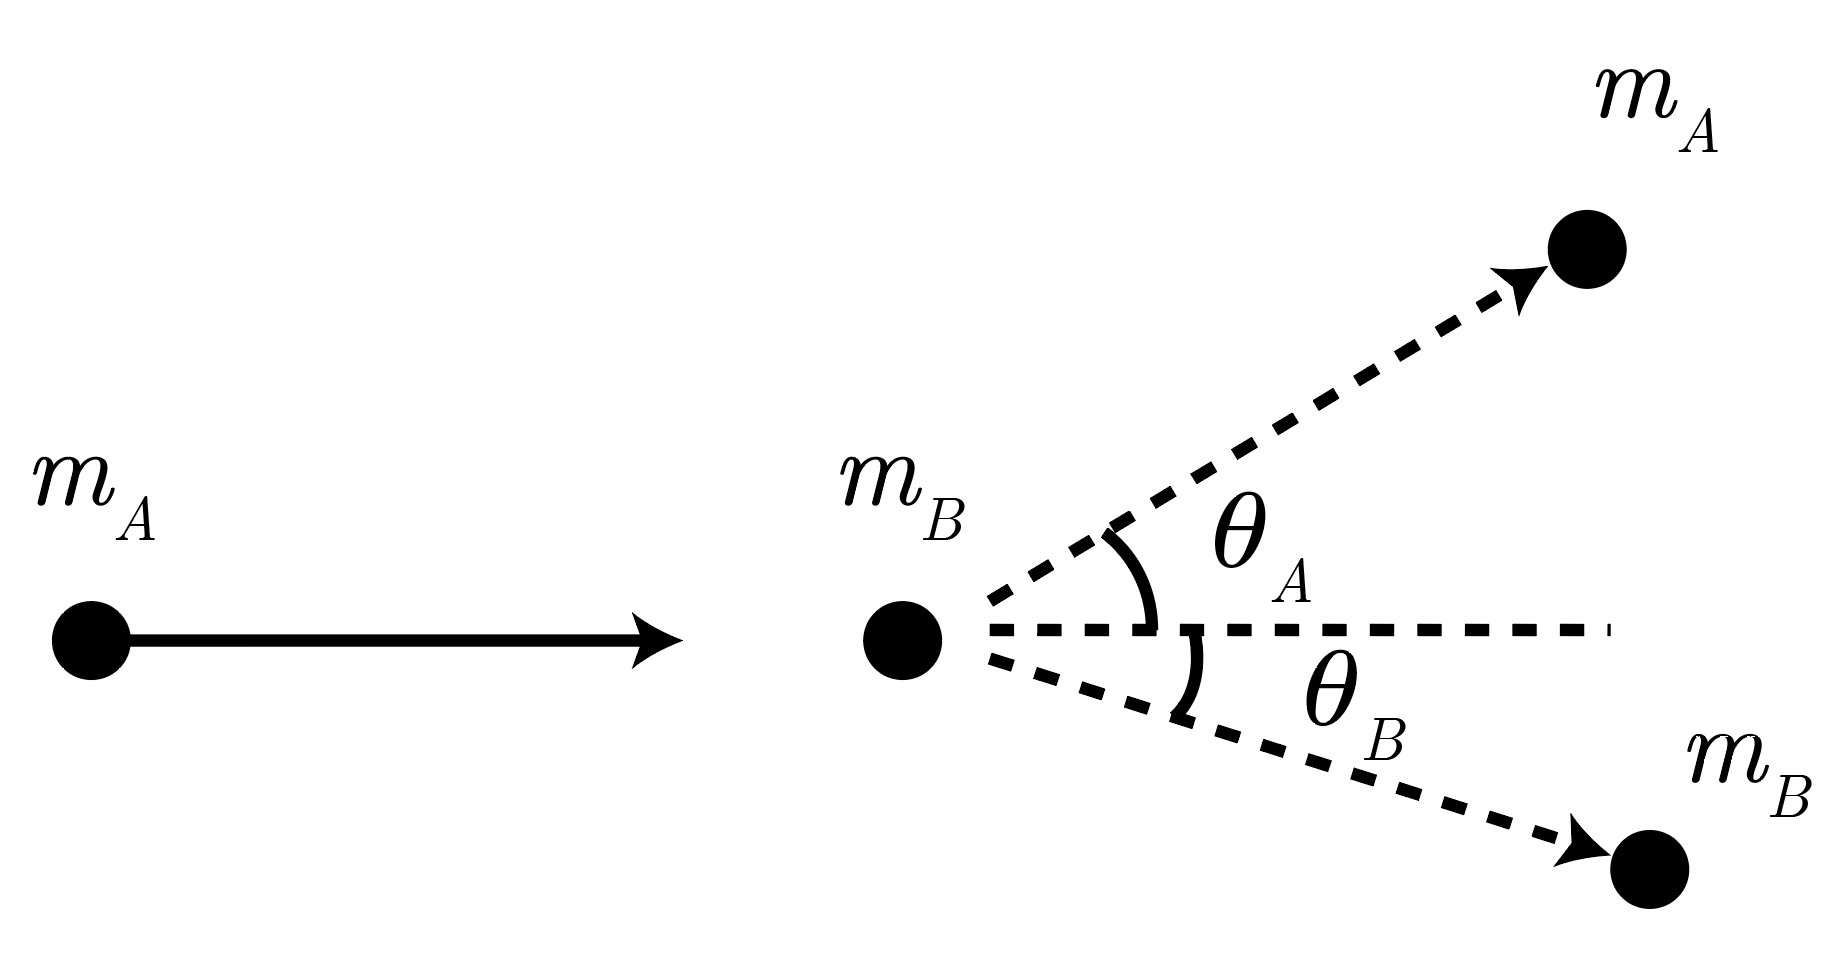
\includegraphics[scale=0.2]{elastic2}
    \end{center}
    \begin{anum}
        \item Find $\cos\theta_A$ as a function of $E_A'$.
        \item Find the maximum possible deflection of $m_A$ after the collision if $m_A>m_B$.
    \end{anum}
\end{prob}

\begin{sol}
    \begin{anum}
        \item Let $P_A$, $P_B$, $P_A'$, and $P_B'$ correspond to $m_A$ before, $m_B$ before, $m_A$ after, and $m_A$ after, respectively. Then, $P_A+P_A=P_A'+P_B'$. Isolating $P_B'$ and squaring both sides, \begin{align*}
    P_B'^2&=P_A^2+P_B^2+P_A'^2+2(P_AP_B-P_AP_A'-P_BP_A')\\
    m_B^2&=m_A^2+m_B^2+m_A^2+2(E_Am_B-(E_AE_A'-p_Ap_A'\cos\theta_A)-E_A'm_B)\\
    \cos\theta_A&=\frac{E_AE_A'+E_A'm_B-E_Am_B-m_B^2}{p_Ap_A'}
\end{align*}Note that $p_A=\sqrt{E_A^2-m_A^2}$ and $p_A'=\sqrt{E_A'^2-m_A^2}$ so we finish: $$\cos\theta_A=\boxed{\frac{(E_A+m_B)(E_A'-m_B)}{\sqrt{(E_A^2-m_A)(E_A'^2-m_A^2)}}}$$
\item Taking the derivative of the right side with respect to $E_A'$ and setting to 0, $$\frac{1}{\sqrt{{E_A'}^2-m_A^2}}-\frac{(E_A'-m_B)E_A'}{({E_A'}^2-m_A^2)^{3/2}}=0\Rightarrow E_A'=\frac{m_1^2}{m_2}$$Plugging this in, the maximal deflection is $$\theta_A=\boxed{\cos^{-1}\left(\frac{E_A+m_B}{m_A}\sqrt{\frac{m_A^2-m_B^2}{E_A^2-m_A^2}}\right)}$$
    \end{anum}
\end{sol}

\begin{prob}
    A charge $Q$ is fixed and a ball of mass $m$ and charge $-q$ orbits around it due to electrostatic attraction. 
    \begin{anum}
        \item Ignoring relativity, the orbit of the ball is an ellipse by Kepler's laws. If we account for relativity, is the orbit still an ellipse?
        \item Now assume the ball orbits in a circular orbit at speed $v$. Accounting for relativity, what is the radius of the orbit?
    \end{anum}
\end{prob}

\begin{sol}
    \begin{anum}
        \item The Lorentz force is unaffected by relativity. However, Newton's second law is affected by the $\gamma^3$ term, so the parallel component of the ball's acceleration under the Lorentz force doesn't follow the classical effect. Thus, the orbit is \fbox{no longer an ellipse}.
        \item The force acting on the ball is the standard electrostatic attraction: $$F=\frac{Qq}{4\pi\epsilon_0r^2}$$Using the definition of force, $$\frac{Qq}{4\pi \epsilon_0 r^2}=\frac{d(\gamma mv)}{dt}=\gamma m\frac{dv}{dt}=\gamma m\frac{v^2}{r}$$Note that $\gamma$ is a constant because the \textit{magnitude} of the velocity always stays the same. Thus the radius is $$r=\boxed{\frac{Qq\sqrt{1-v^2}}{4\pi\epsilon_0mv^2}}$$
    \end{anum}
\end{sol}

\begin{prob}[Morin]
A relativistic dustpan of mass $M$ is given a speed $V$. Immediately in front of it along the floor is dust of linear mass density $\lambda$. The dustpan begins gathering the dust. \begin{anum}
    \item At the instant the speed of the dustpan is $v$, find the rate at which the mass of the dustpan-dust system is increasing.
    \item Find $v(x)$, $v(t)$, and $x(t)$. 
\end{anum}
\end{prob}

\begin{sol}
    \begin{anum}
        \item Let the dustpan have mass $M'$ at this moment. The 4-momentum of the dustpan is $P_1=(\gamma M',\gamma M'v)$, and the 4-momentum of the small piece of dust it will pick up is $P_2=(\lambda v \,dt,0)$. The mass after the dust is absorbed is $$m=\sqrt{(P_1+P_2)^2}=\sqrt{M'^2+(\lambda v \,dt)^2+2M'\lambda v \, dt}\approx \sqrt{M'^2+2\gamma M'\lambda v \, dt}\approx M'+\gamma \lambda v\, dt$$ where in the last step we used a Taylor approximation. Thus the rate of increase in mass is $$\mu = \gamma\lambda v=\boxed{\frac{\lambda v}{\sqrt{1-v^2}}}$$
        \item The total momentum $p=\gamma_VMV$ of the system is conserved. Note that after traveling a distance $x$, the energy of the system is $E(x)=\gamma_VM+\lambda x$. As a result, $$v(x)=\frac{p}{E(x)}=\boxed{\frac{\gamma_V MV}{\gamma_VM+\lambda x}}$$ Now, to find $v(t)$, notice that since $dE/dx=\lambda$, $dE/(v\, dt)=d(p/v)/v\, dt=(-p/v^3)(dv/dt)=\lambda.$ Integrating, $$-\int_V^v \frac{p}{v^3}dv=\int_0^t\lambda dt\Rightarrow \frac{p}{v^2}-\frac{p}{V^2}=2\lambda t\Rightarrow v(t)=\boxed{\frac{V}{\sqrt{1+(2V\lambda t/\gamma_V M)}}}$$Integrating to obtain $x(t)$ yields $$x(t)=\boxed{\frac{\gamma_V M}{\lambda}\left(\sqrt{1+\frac{2v\lambda t}{\gamma_V M}}-1\right)}$$
    \end{anum}
\end{sol}

\begin{prob}[Morin]
    Consider a dumbbell made of two equal masses, $m$. The dumbbell spins around, with its center pivoted at the end of a stick. If the speed of the masses is $v$, then the energy of the system is $2\gamma m$. Treated as a whole, the system is at rest. Therefore, the mass of the system must be $2\gamma m$. (Imagine enclosing it in a box, so that you can’t see what’s going on inside.) Convince yourself that the system does indeed behave like a mass of $M = 2\gamma m$, by pushing on the stick (when the dumbbell is in the “transverse” position shown in the figure) and showing that $F= dp/dt =Ma$.
    \begin{center}
        
\includegraphics[scale=0.2]{morin1}
    \end{center}
\end{prob}

\begin{sol}
    Let the speed of the stick go from zero to $\epsilon$, where $\epsilon \ll v$. Then the final speeds of the two masses are obtained by relativistically adding or subtracting $\epsilon$ from $v$. (Assume that the time involved is small, so that the masses are still essentially moving horizontally.) The effective $\gamma$ is $\gamma_\epsilon\gamma_v(1+\epsilon v)$, so the final momenta of the two masses have magnitudes $\gamma_\epsilon \gamma_v(v\pm \epsilon)m$. But since $\epsilon$ is small, we can set $\gamma \epsilon \approx 1$, to first order. Therefore, the forward-moving mass has momentum $\gamma_v(v + \epsilon)m$, and the backward-moving mass has momentum $\gamma_v(v-\epsilon)m$. So the net increase in momentum is $\Delta p=2\gamma m\epsilon$, where $\gamma=\gamma_v$. Hence, $$F=\frac{\Delta p}{\Delta t}=2\gamma m\frac{\epsilon}{\Delta t}=2\gamma ma\equiv Ma$$
\end{sol}

\begin{prob}
    A relativistic string of length $\ell$ and tension $T$ is attached to a mass $M$ on one end and a mass $m$ on the other end. The masses are released from rest. Find the time it takes for the masses to collide. 
\end{prob}

\begin{sol}
    Let's examine the moment right before the masses collide. The total energy between the masses is $E_1+E_2=M+m+T\ell$, and the momenta of the masses must sum to 0, so $$E_1^2-M^2=E_2^2-m^2$$. Rearranging the second equation and dividing by the first, we get a system of two linear equations: \begin{gather*}
        E_1+E_2=M+m+T\ell\\
        E_1-E_2=\frac{M^2-m^2}{M+m+T\ell}
    \end{gather*}which solves as $$E_1=\frac12\left(M+m+T\ell+\frac{M^2-m^2}{M+m+T\ell}\right)$$ The time it takes to collide is $p_1/T$, so $$t=\frac{p_1}{T}=\frac{\sqrt{E_1^2-M^2}}{T}=\boxed{\frac{\sqrt{T\ell(2M+T\ell)(2m+T\ell)(2M+2m+T\ell)}}{2T(M+m+T\ell)}}$$
\end{sol}


\begin{prob}[NBPhO]
A photon rocket is accelerated by a laser beam sent from the ground: the rocket’s mirror reflects the photons in the exact opposite direction. The rocket’s rest mass $M_0$ did not change during the ride. The total energy of the photons emitted by the laser (and later reflected by the rocket) is $\alpha M_0c^2$. The laser power is constant over time. 
\begin{anum}
    \item What speed $v$ does the rocket reach if $\alpha=1\times 10^{-6}$?
    \item What speed $v$ does the rocket reach if $\alpha=1$? Hint: Use one 4-vector to represent all of the emitted photons. 
    \item How many times does the rocket's acceleration, as perceived by passengers (i.e. the inertial force acting on them) differ at the beginning and at the end of the acceleration if $\alpha=1$? Express the answer in terms of the rocket’s final speed $v$.
\end{anum}
\end{prob}

\begin{sol}
    See solutions \href{https://nbpho.ee/wp-content/uploads/2022/NBPhO_2022_solutions.pdf}{here} (problem 3). 
\end{sol}

\subsection{Challenge Problems}

\begin{prob}[Morin]
Two equal masses are connected by a massless string with tension $T$. The masses are constrained to move with speed $v$ along parallel lines. The constraints are then removed, and the masses are drawn together. They collide and make one blob which continues to move to the right. Is the following reasoning correct? If your answer is ``no," state what is invalid about whichever of the four sentences is/are invalid.\\ 
``The forces on the masses point in the $y$ direction. Therefore, there is no change in the momentum of the masses in the $x$ direction. But the mass of the resulting blob is greater than the sum of the initial masses (because they collide with some relative speed). Therefore, the speed of the resulting blob must be less than $v$ (to keep $p_x$ constant), so the whole apparatus slows down in the $x$ direction."
\begin{center}

\includegraphics[scale=0.2]{morin2}
\end{center}
\end{prob}
\begin{sol}
    The first sentence is wrong. As the masses begin moving towards each other, their directions of motion become tilted at an angle to the horizontal. Then, the transverse component of tension relative to the direction of motion scales by $1/\gamma$ while the parallel component doesn't scale, so the net force ends up deviating from the vertical direction, resulting in a decrease in the momentum in the $x$ direction. 
\end{sol}

\begin{prob}[IPhO]
    Try Problem 1 from IPhO 1995 \href{https://s3.eu-central-1.amazonaws.com/physprob.com/files/ipho/1995_Australia_p1.pdf}{here}. Part (b) is excellent practice with experimental physics!
\end{prob}

\begin{sol}
    See solutions \href{https://s3.eu-central-1.amazonaws.com/physprob.com/files/ipho/1995_Australia_p1Sol.pdf}{here}.
\end{sol}

\begin{prob}[IPhO]
Try Part A of Problem 1 from IPhO 2003 \href{https://s3.eu-central-1.amazonaws.com/physprob.com/files/ipho/2003_Taiwan_p3.pdf}{here}. This is probably the hardest relativistic dynamics olympiad problem ever written, so approach with caution!
\end{prob}

\begin{sol}
    See solutions \href{https://s3.eu-central-1.amazonaws.com/physprob.com/files/ipho/2003_Taiwan_p3Sol.pdf}{here}.
\end{sol}


\subsection{USAPhO Practice}

\begin{prob}[USAPhO 2023 B2]
A space program wants to accelerate a spaceship of mass $m = 100 \,\unit{kg}$ to relativistic speeds to observe distant stars. The ship is propelled by light produced by lasers on Earth, with total power $P = 6 \times 10^{12}\,\unit{W}$. The light evenly impacts a sail on the spaceship, and reflects off the sail directly back towards the Earth. Neglect the orbital motion of the Earth, and give all your answers in the frame of the Earth.

\begin{anum}
    \item What is the force on the spaceship when the spaceship has speed $v$?
    \item How long will it take to accelerate the spaceship to speed $v_f = 3c/5$, in seconds? You may use the following integral: $$\int \frac{dx}{(1-x)^2\sqrt{1-x^2}}=\frac{(2-x)\sqrt{1+x}}{3(1-x)^{3/2}}+C$$
    \item At the moment the spaceship reaches this speed, how much total energy has been used to power the lasers, in Joules?
\end{anum}
\end{prob}

\begin{sol}
    See solutions \href{https://www.aapt.org/physicsteam/upload/2023-USAPhO-solutions.pdf}{here}.
\end{sol}

\begin{prob}
    In this problem we study the dynamics of relativistic strings. In all of the parts below, the relativistic strings have tension $T$ in their rest frame.
    \begin{anum}
        \item A string of length $L$ connects two masses $m$ initially moving at speeds $v$ perpendicularly to the string. Find the tension in the string in the lab frame. 
        \begin{center}
            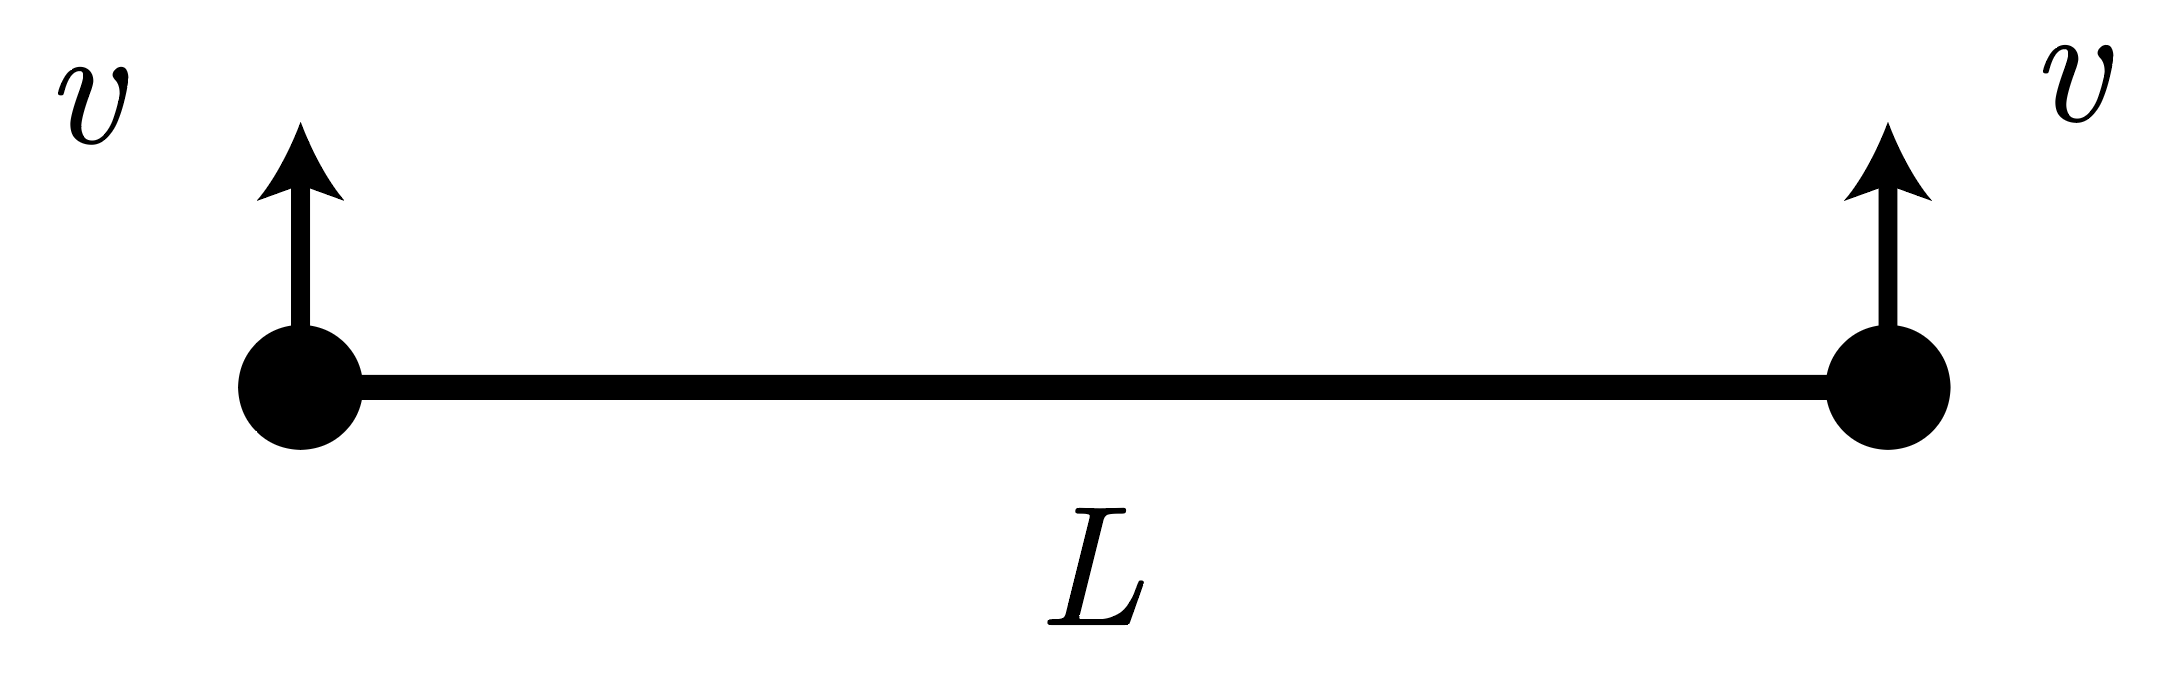
\includegraphics[scale=0.15]{string1}
        \end{center}
        \item Find the energy of the string from part (a) in the lab frame.
        \item In the lab frame, find the amount of time it takes for the masses to collide. 
        \item Now, suppose the masses are replaced by quarks each with energy $E$ directed with velocities at a 45$^\circ$ angle outward as shown. Assume $E,TL\gg \mu$, the mass of one quark. Find the time it takes for them to collide. 
        \begin{center}
            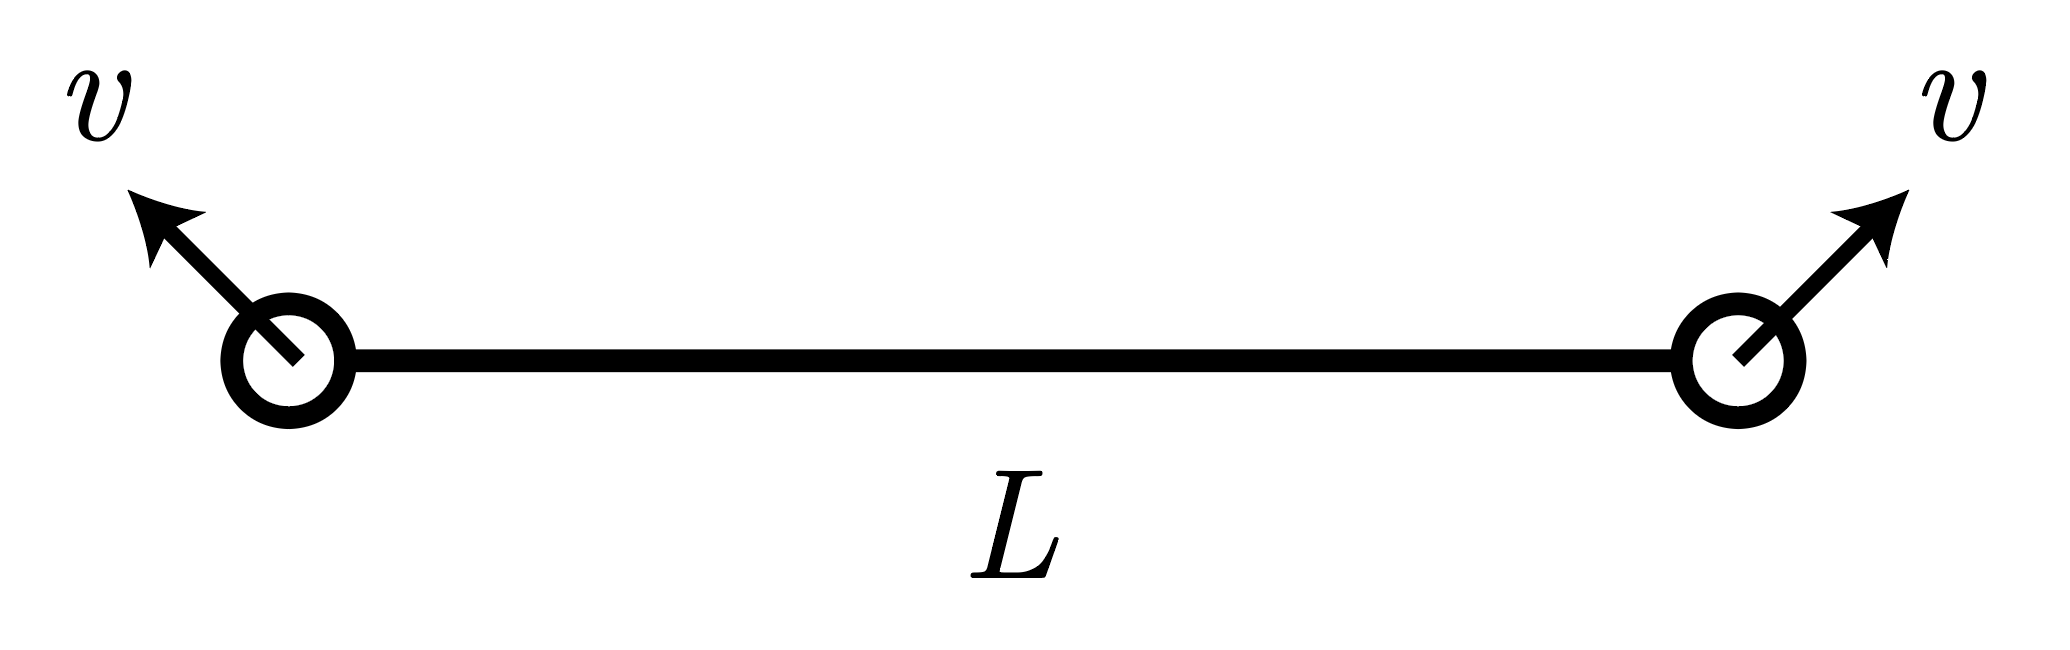
\includegraphics[scale=0.15]{string3}
        \end{center}
        \item Now assume the quark on the left starts with energy $E_1$, the other quark starts with energy $E_2>E_1$, and the velocities are still directed at the 45$^\circ$ angle. Assume still that $E_1,E_2\gg \mu$. Sketch the paths taken by the quarks in the lab frame up until the point they collide. Label all relevant lengths so the paths are well-defined, but you don't need to find any time measurements.
    \end{anum}
\end{prob}

\begin{sol}
    \begin{anum}
        \item Using the transverse transformation of force, $$T'=\frac{T}{\gamma}=\boxed{T\sqrt{1-v^2}}$$
        \item The string has energy $TL$ in its rest frame and zero momentum. By the Lorentz transformations of energy, the energy in the lab frame is $$E'=\gamma E=\boxed{\frac{TL}{\sqrt{1-v^2}}}$$
        \item Let's first find the time in the rest frame. The energy of each mass right before the collision is $m+(TL/2)$, so their momenta are equal to $p=\sqrt{E^2-m^2}=\sqrt{TLm+(TL/2)^2}$. Then, $t=p/T$. By time dilation, $t'=\gamma t$, so $$t'=\gamma\frac{p}{T}=\boxed{\sqrt{\frac1{1-v^2}\left(\frac{Lm}{T}+\frac{L^2}{4}\right)}}$$
        \item Since the quarks have very small rest mass compared to the energies we're dealing with, we can assume they are always traveling at speed $c$. In the frame moving upward at $c/\sqrt2$ (with $\gamma=\sqrt2$), the quarks will have speeds $c$ directed parallel to the string (this can be found via transverse velocity addition, or by the fact that the speed of light doesn't depend on frame). To find the energy of the quarks in this new frame, we can use the invariance of the inner product, so $$(E, E/\sqrt2,E\sqrt2,0)\cdot(E, -E/\sqrt2,E\sqrt2,0)=(E',E',0,0)\cdot(E',-E',0,0)\Rightarrow E'=\frac{E}{\sqrt2}$$Alternatively, we could have transformed to the rest frame via the Lorentz transformations. As a result, by conservation of energy, the string will extend to a length given by $$TL'=TL+2E'\Rightarrow L'=L+\frac{E\sqrt2}{T}$$ before the quarks turn around and eventually collide. During this time, the speed of the quarks is always $c$ (or 1, in the units $c=1$), so the total time the process takes in the rest frame is $$t=\frac{L'-L}{2c}+\frac{L'}{2c}=\frac{L}{2}+\frac{E\sqrt2}{T}$$
        By time dilation, we shift back into the lab frame with $t'=\gamma t=\sqrt2 t$: $$t'=\boxed{\frac{L}{\sqrt2}+\frac{2E}{T}}$$
        \item In the frame moving upward at $c\sqrt2$, the mass on the left will stop first and turn back after traveling a distance $E_1\sqrt2/T$, and the mass on the right will then stop later after traveling a distance $E_2\sqrt2/T$. There is no transverse length contraction, so this is the horizontal distance traveled in the lab frame. The vertical component is the same, because the movement at the 45$^\circ$ angle. When the masses turn, they will move toward each other at $45^\circ$ inward in the lab frame until they collide. Thus, the diagram should look something like the following: \begin{center}
            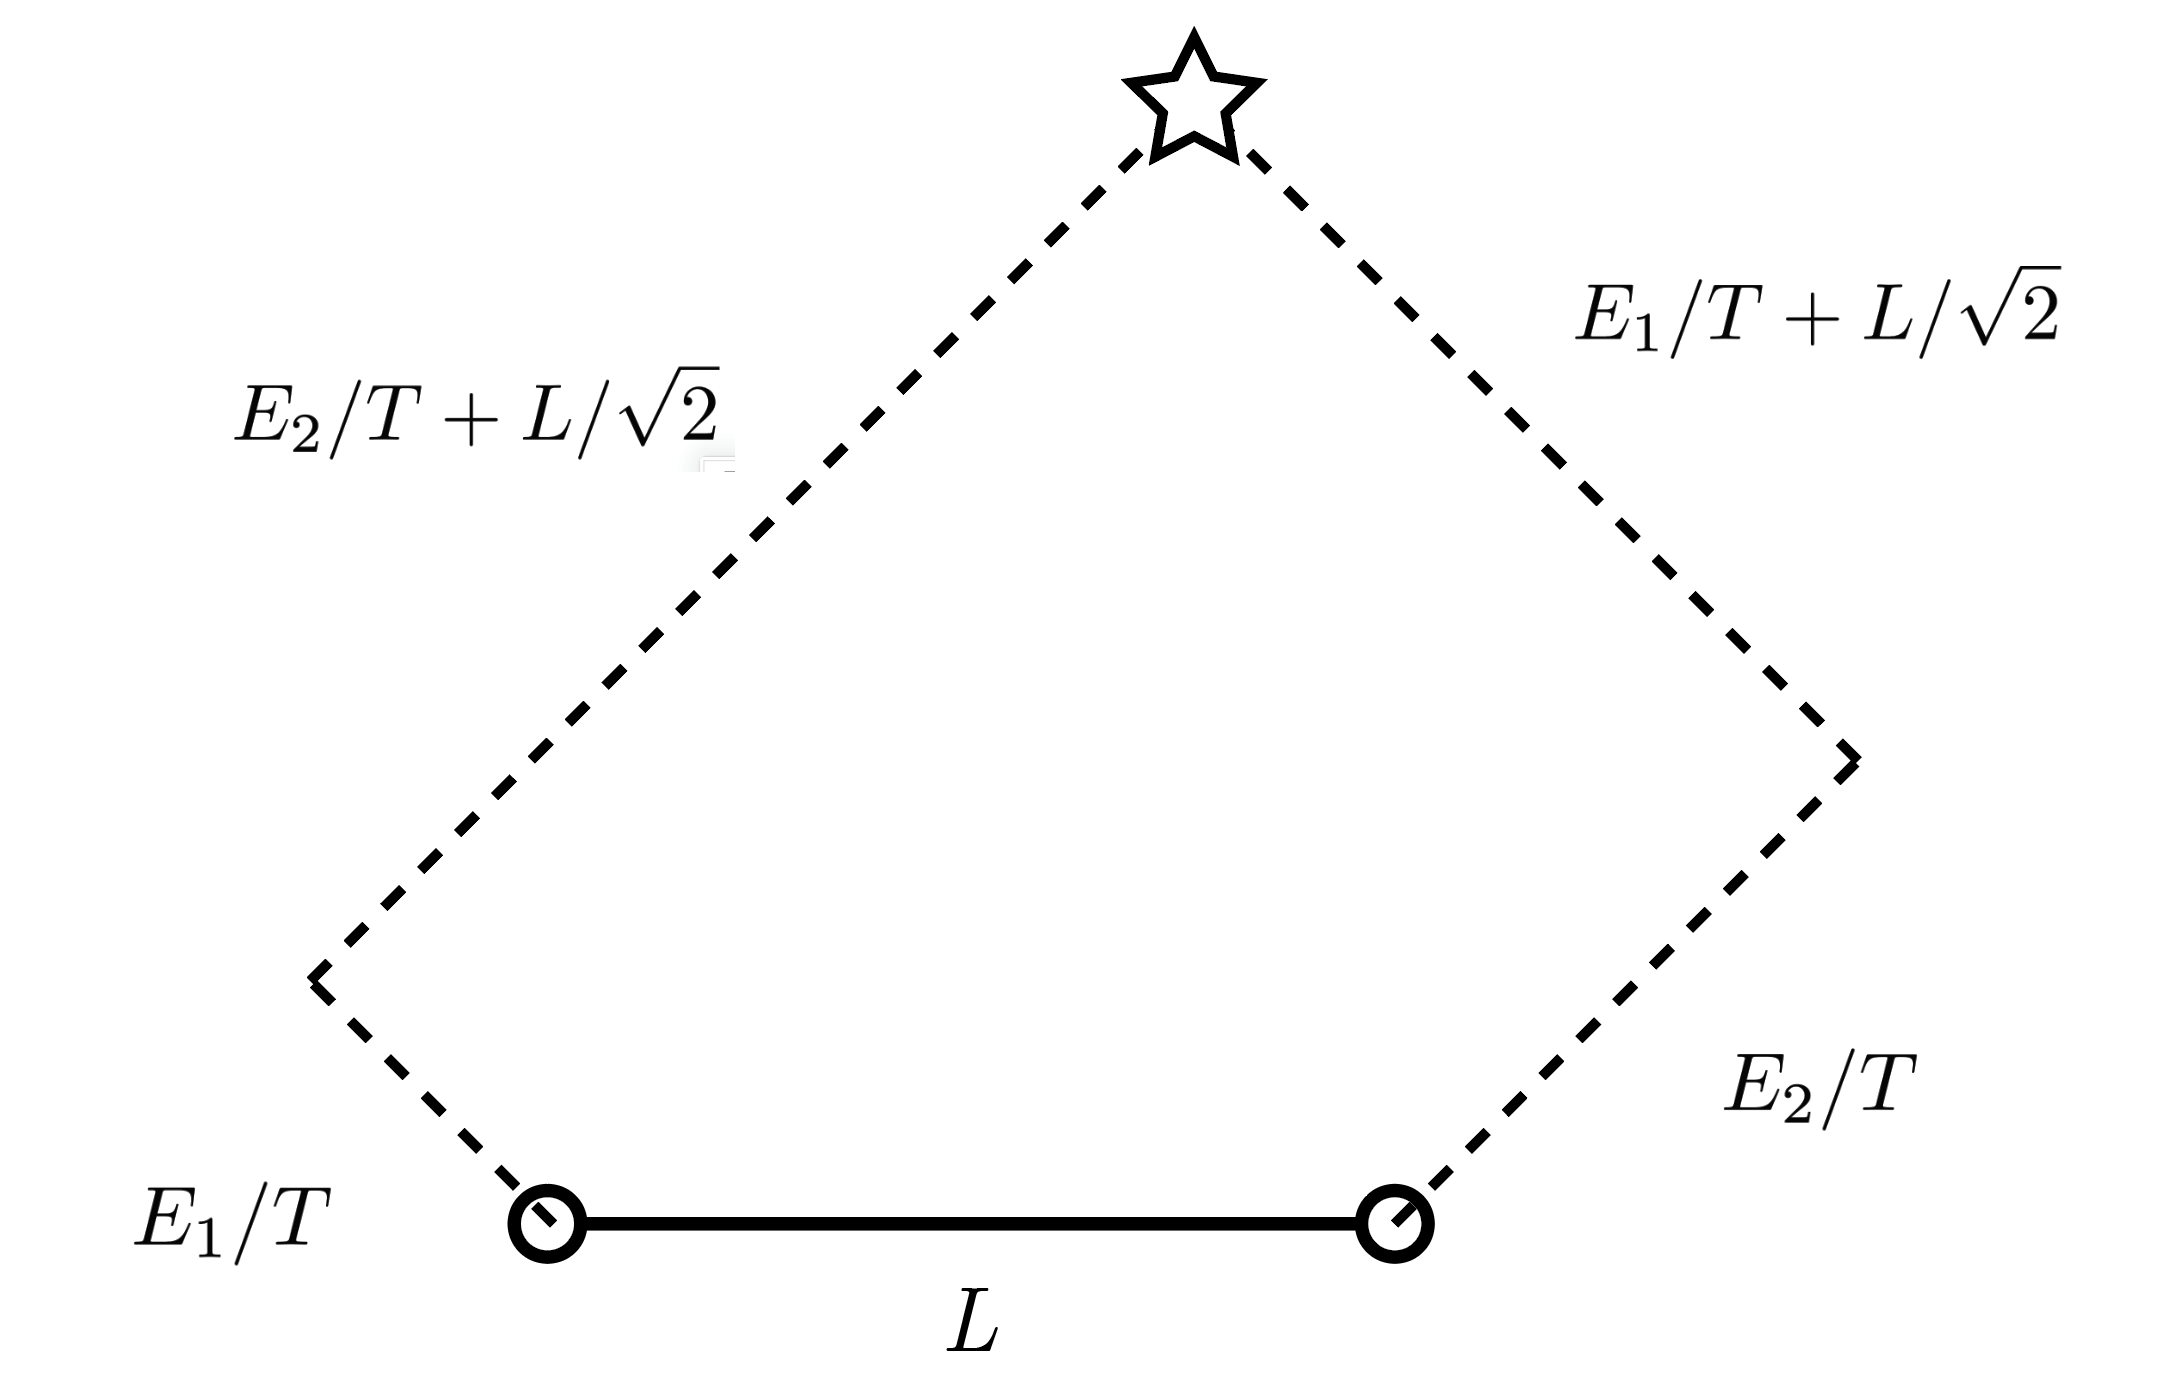
\includegraphics[scale=0.3]{heyyo}
        \end{center}
    \end{anum} 
\end{sol}

\end{document}